\newpage
\subsection*{Task 2}

\subsubsection*{b)}

\begin{figure}[h!]
    \centering
    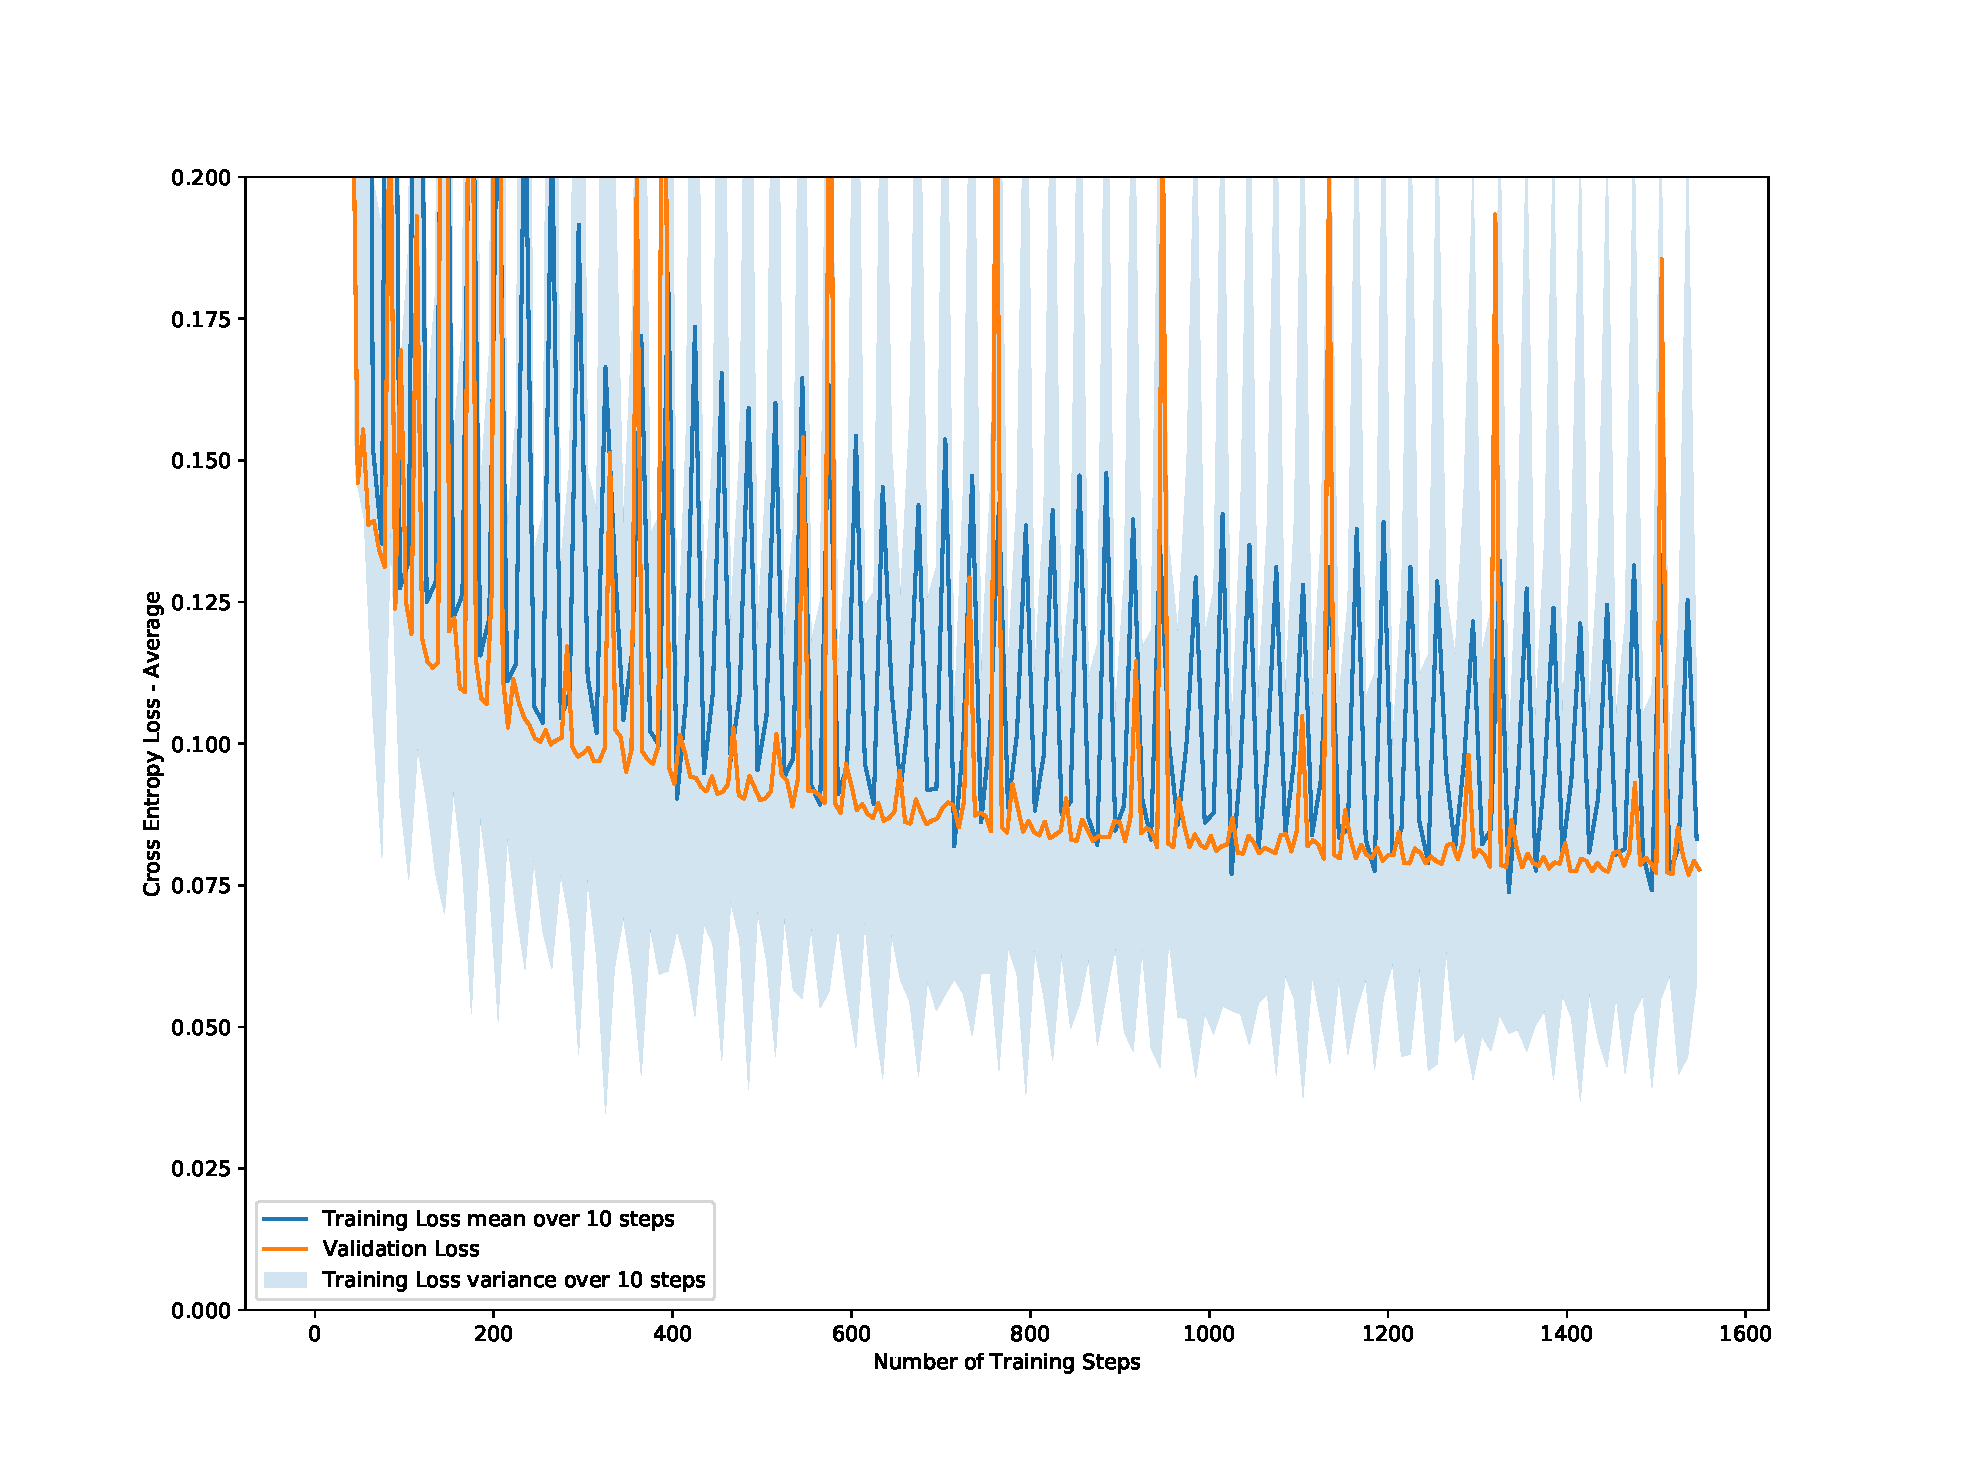
\includegraphics[clip, trim=0cm 0cm 0cm 0cm,width=0.85\textwidth]{figures/Task2b.pdf}
    \caption{Training and validation loss over training.}
    \label{fig:task2:train_val_loss}
\end{figure}

\subsubsection*{c)}

\begin{figure}[h!]
    \centering
    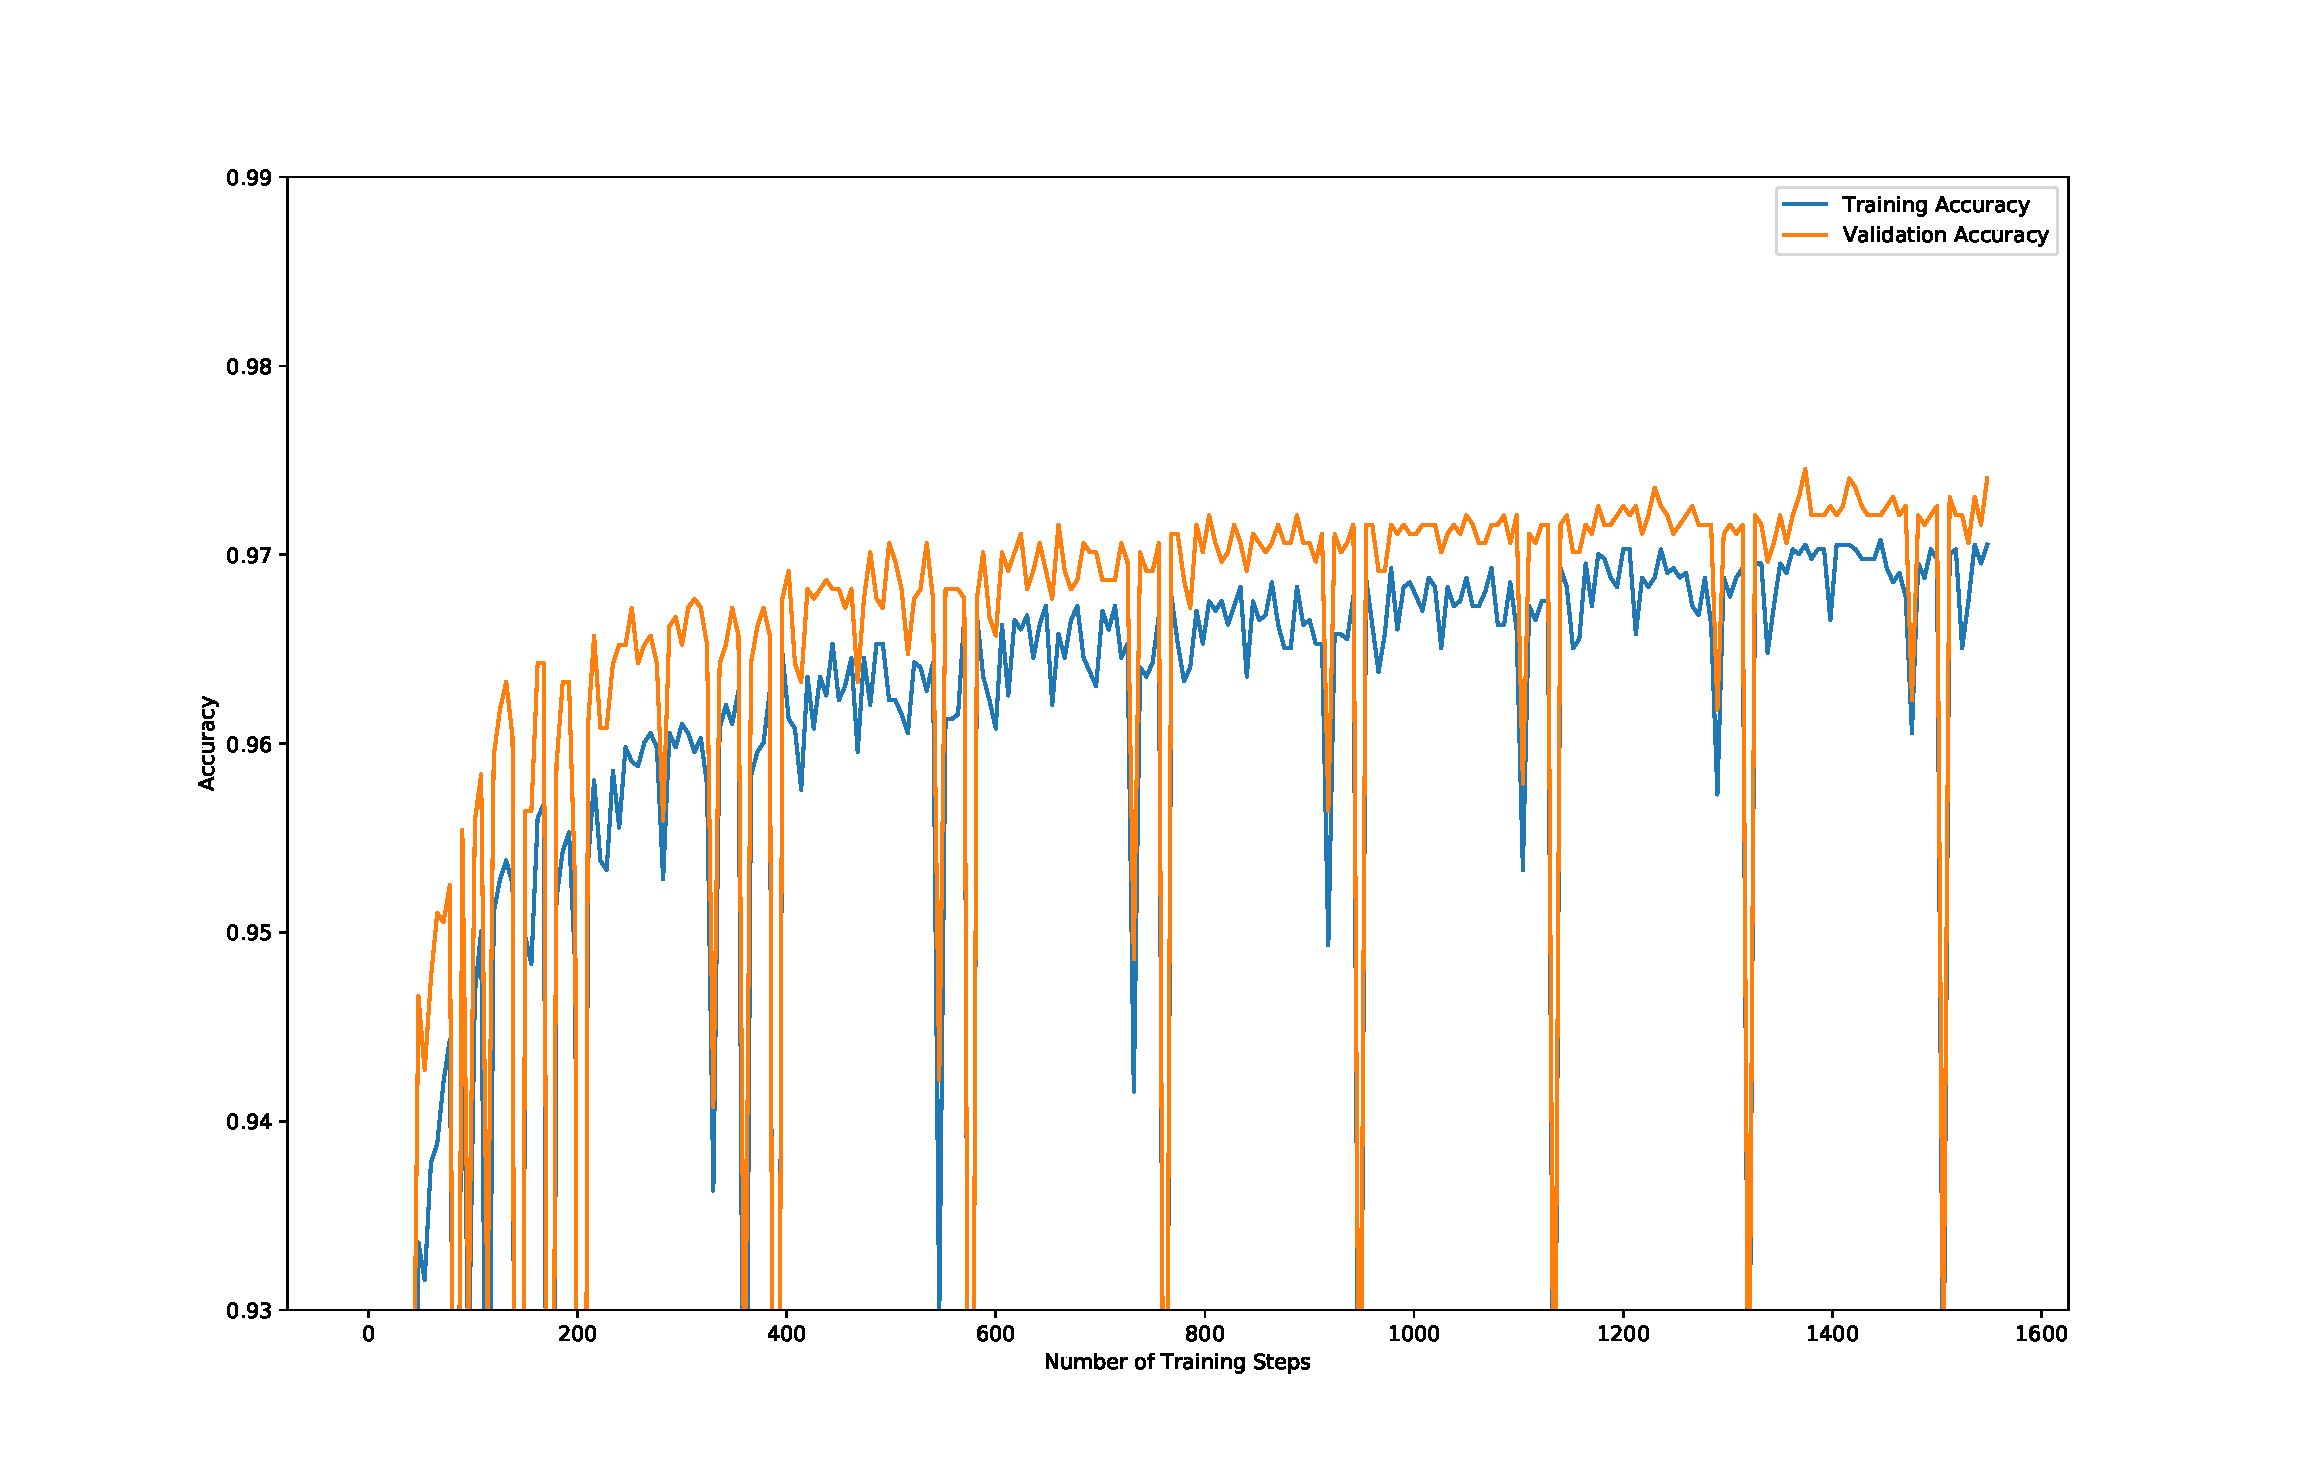
\includegraphics[clip, trim=0cm 0cm 0cm 0cm,width=0.85\textwidth]{figures/Task2c.pdf}
    \caption{Accuracy on training and validition set over training.}
    \label{fig:task2:accuracy}
\end{figure}

\subsubsection*{d)}

Early stopping kicked in after 35 epochs. Side note: one should perhaps use the weights at the validation loss minimum as final weights, but I have not implemented this in the code, as it does not seem the "Starter code" was made with this in mind. The final weights are therefore the weights at the stopping criteria.

\subsubsection*{e)}

\begin{figure}[h!]
    \centering
    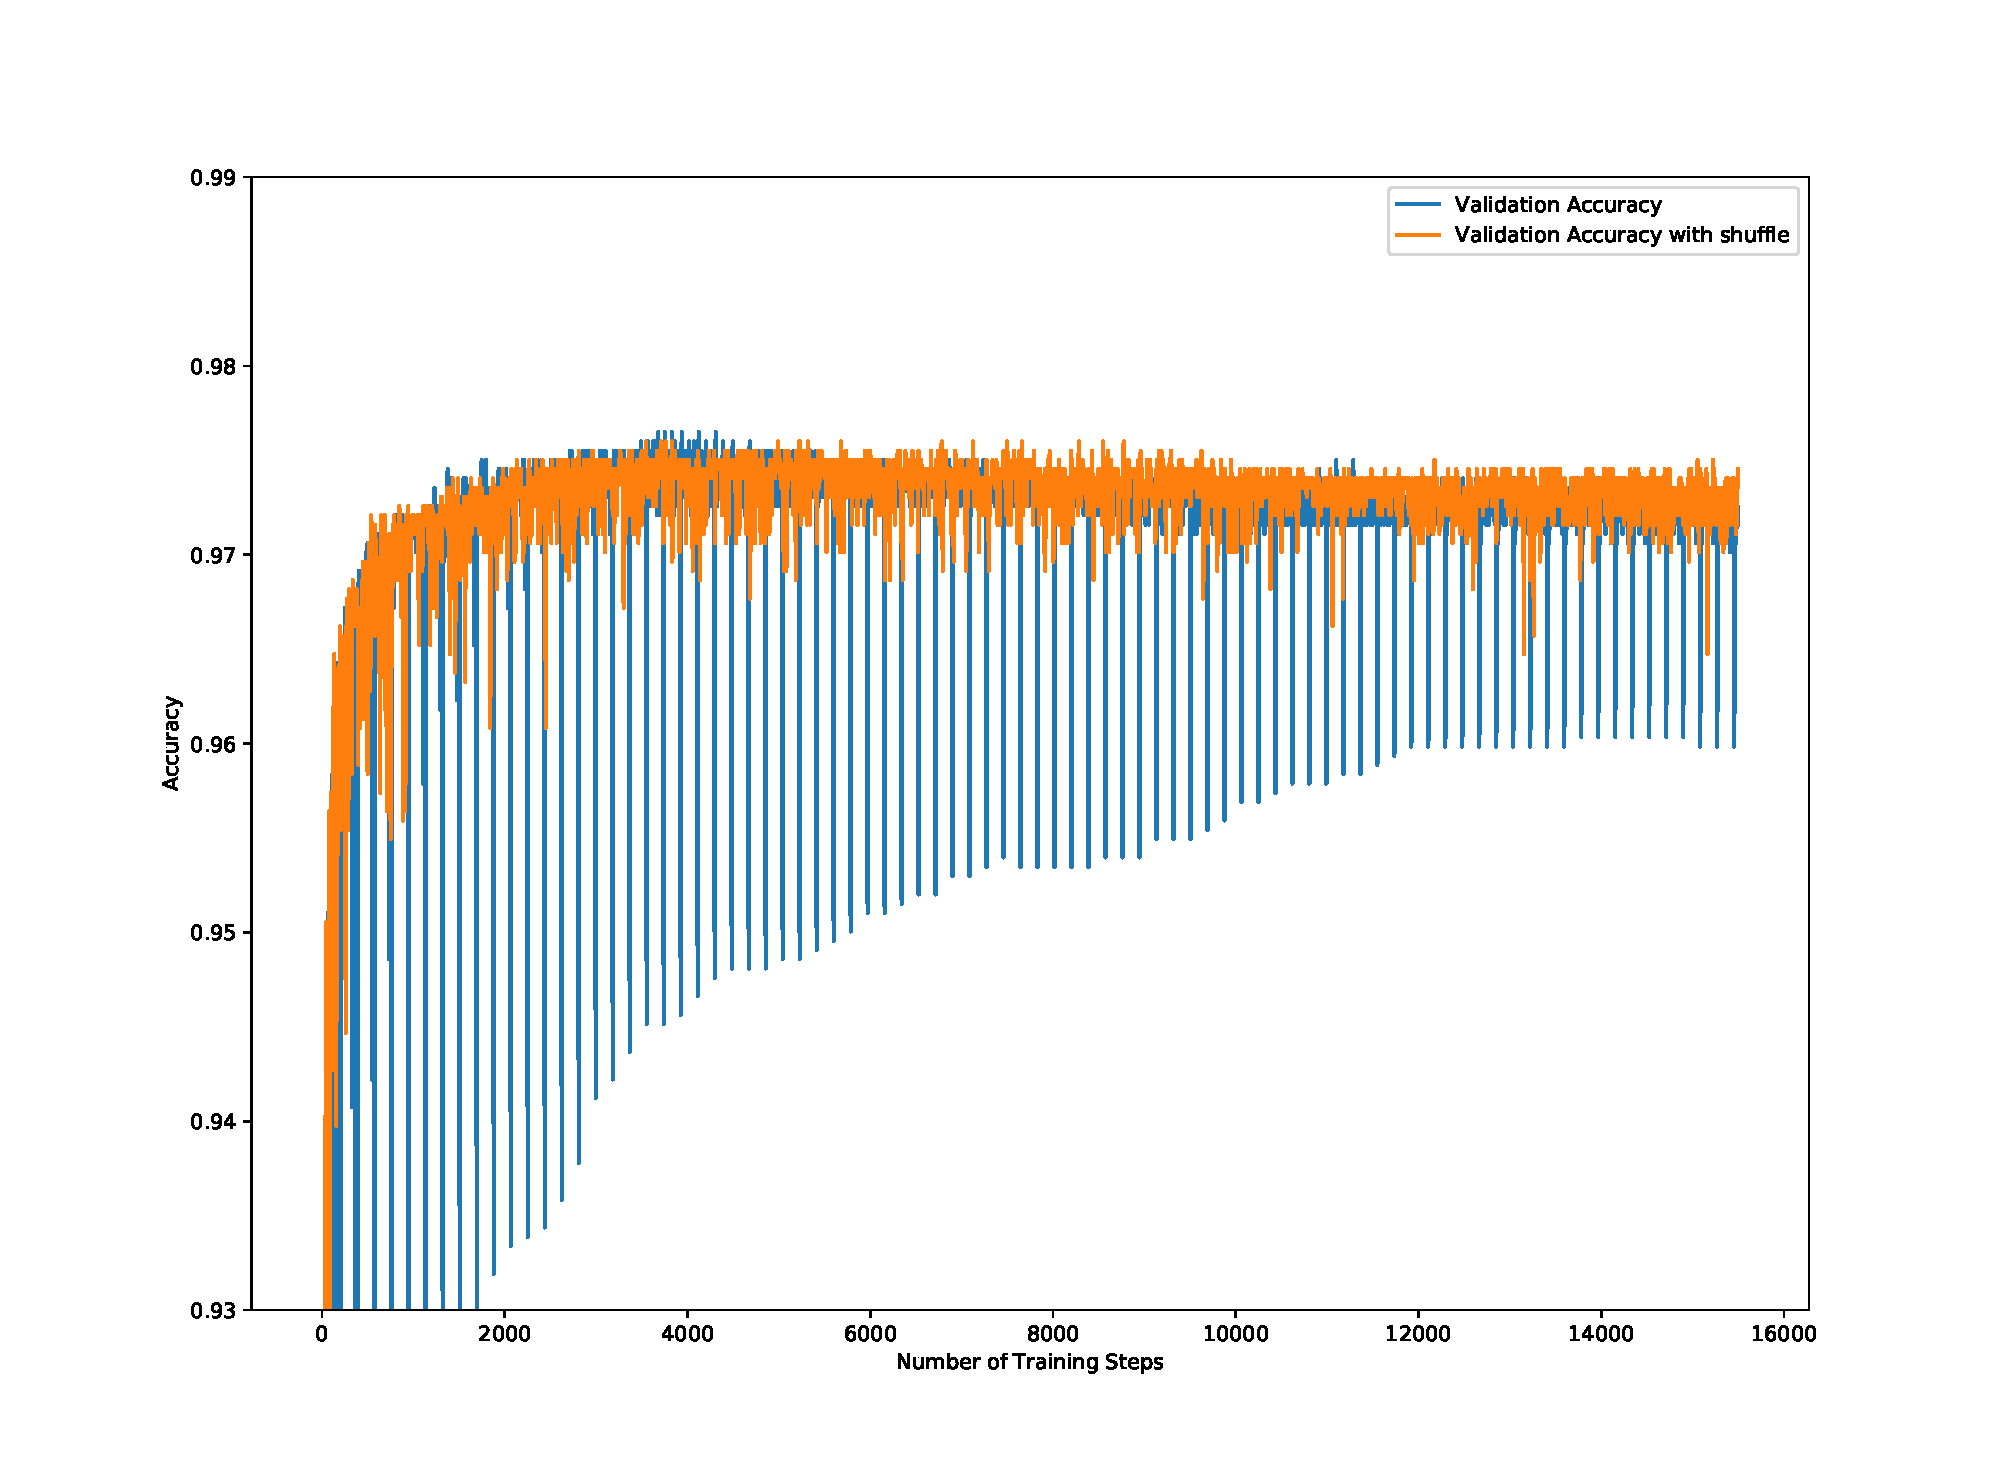
\includegraphics[clip, trim=0cm 0cm 0cm 0cm,width=0.85\textwidth]{figures/Task2e.pdf}
    \caption{Accuracy on validation set with and without dataset shuffling. Early stopping is turned off to better see the difference.}
    \label{fig:task2:shuffle}
\end{figure}

From \cref{fig:task2:shuffle} we see that the validation accuracy has less spikes with dataset shuffling than without. We also see that the spikes come periodically, and by closer inspection, the spikes are seen to come from batch indice [2304, 2431]. This may indicate that this specific batch is not representing the validation set well, and training on this batch will therefore give worse accuracy on the validation set, as the weights are updated to best fit this specific batch. When the data is shuffled, the training step will train over a more generalized set of data that represents the overall distribution of data better. The "poor" batch will effectively no longer exist, and we get the benifit of training over a larger distribution of data while still doing batch gradient descent.
